\documentclass{article}
%\usepackage{geometry}
%\geometry{top = 1in, bottom = 1in, left = 1in, right = 1in}
\usepackage[top = 0.7in, bottom = 0.7in, left = 0.7in, right = 0.7in]{geometry}
\usepackage{amsmath,amssymb,amsthm,mathrsfs}
\usepackage{graphicx}
\usepackage{bm}
\usepackage{float}
\usepackage[font=footnotesize,labelfont=bf]{caption}
\usepackage{movie15}
\usepackage{hyperref}

\usepackage{fancyhdr}
\pagestyle{fancy}
\rhead{\footnotesize {09/08/2012 ; MESA version 4442} }
\chead{\footnotesize {Authors: Jared Brooks, Lars Bildsten, Bill Paxton} }
\lhead{\footnotesize {mesa/star/test\_suite/high\_mass} }

\begin{document}
	
	\begin{center}
	  \begin{Large}
	    \textbf{HIGH MASS}\\
	  \end{Large}
	\end{center}

        This test is to show a 110 $M_\odot$ pre-main sequence star evolved to the middle of the main sequence.  Therefore, this test should be cut off when the mass fraction for center hydrogen drops below 0.5 (\texttt{xa\_central\_lower\_limit\_species(1) = 'h1' ; xa\_central\_lower\_limit(1) = 0.5}).\\

        The inlist sets an initial mass of 100 $M_\odot$ and solar metalicity, and then relaxes the mass (\texttt{new\_mass = 110}) and the metallicity (\texttt{new\_Z = 1d-5}).\\

        To the left is the HR-diagram from the run (figure \ref{fig:1}), starting on the lower branch.  To the right is a plot of the evolution of the center temperature and density (figure \ref{fig:2}).

        \begin{figure}[H]
          \begin{minipage}[b]{0.5\linewidth}
	    \centering
	    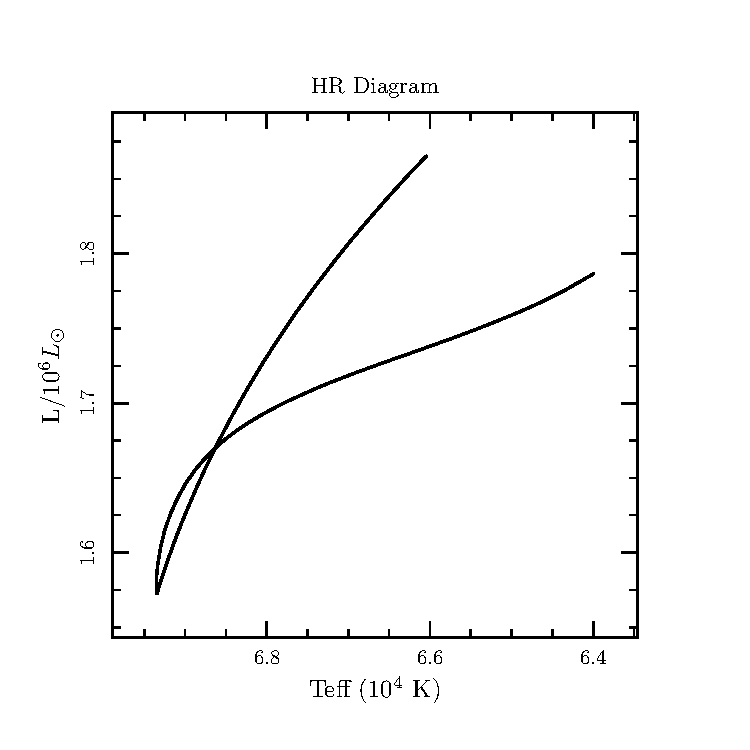
\includegraphics[width = 3.8in]{/Users/jaredbrooks/high_mass/plots_out/HR_Diagram.pdf}
	    \caption{}
	    \label{fig:1}
          \end{minipage}
          \hspace{0cm}
          \begin{minipage}[b]{0.5\linewidth}
            \centering
            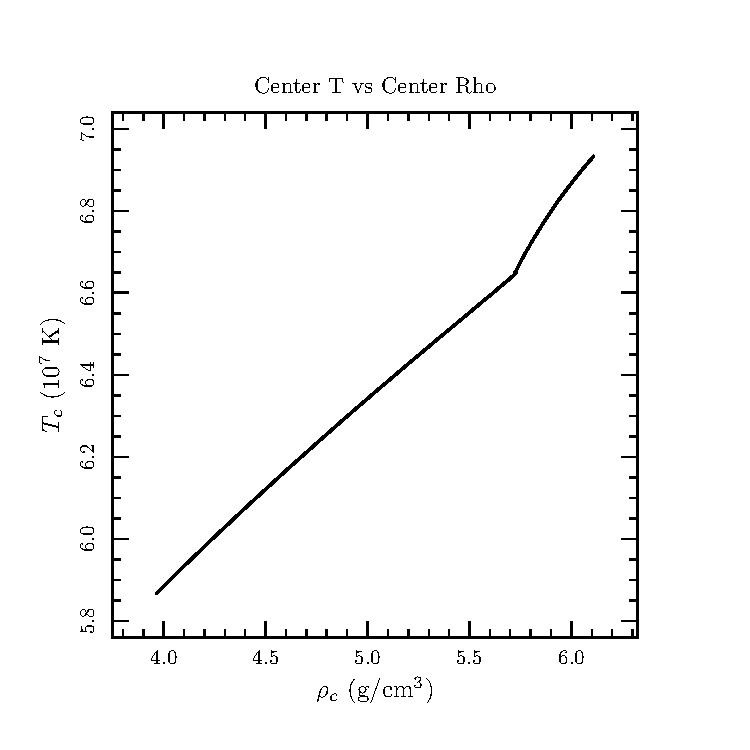
\includegraphics[width = 3.8in]{/Users/jaredbrooks/high_mass/plots_out/Tc_vs_Rhoc.pdf}
            \caption{}
            \label{fig:2}
          \end{minipage}
	\end{figure}

        \pagebreak

        Below are an abundance profile (figure \ref{fig:3}) and a burning rate profile (figure \ref{fig:4}) from the end of the run.

        \begin{figure}[H]
            \begin{minipage}[b]{0.5\linewidth}
            \centering
            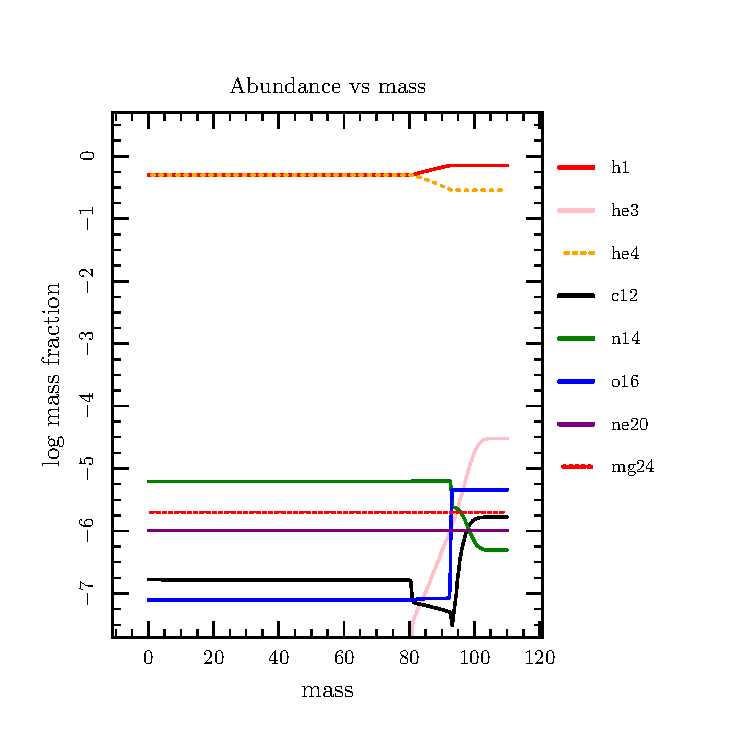
\includegraphics[width = 3.8in]{/Users/jaredbrooks/high_mass/plots_out/Abundance_vs_mass_3.pdf}
            \caption{}
            \label{fig:3}
          \end{minipage}
          \hspace{0cm}
          \begin{minipage}[b]{0.5\linewidth}
            \centering
            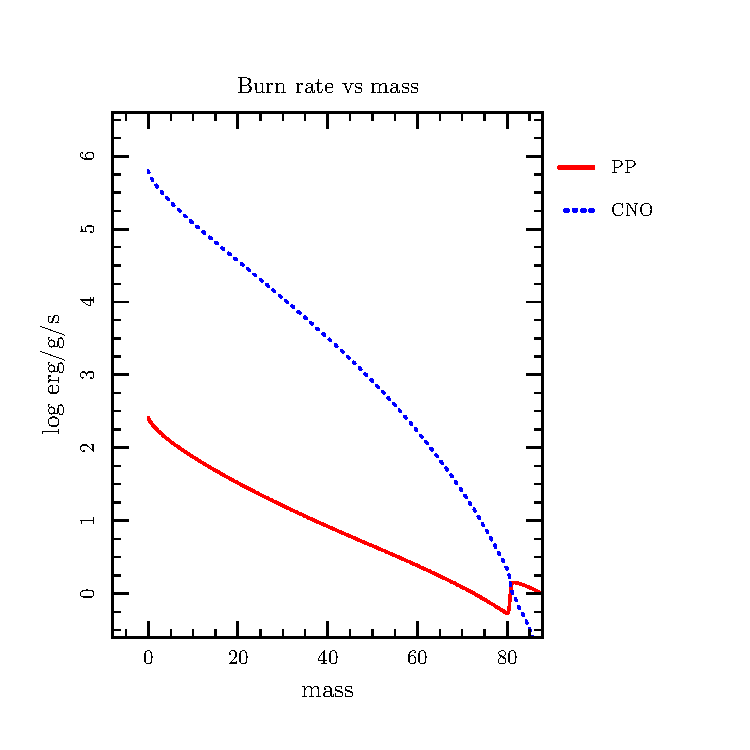
\includegraphics[width = 3.8in]{/Users/jaredbrooks/high_mass/plots_out/Burnrate_vs_mass_3.pdf}
            \caption{}
            \label{fig:4}
          \end{minipage}
        \end{figure}

        \pagebreak

        This final plot (figure \ref{fig:5}) shows a few internal \texttt{MESA} variables, such as the size of the time-step, the number of zones, and the number of retries against the model number in order to give some understanding of how hard \texttt{MESA} is working throughout the run and where some areas of problems/interest might be.

        \begin{figure}[H]
          \centering
          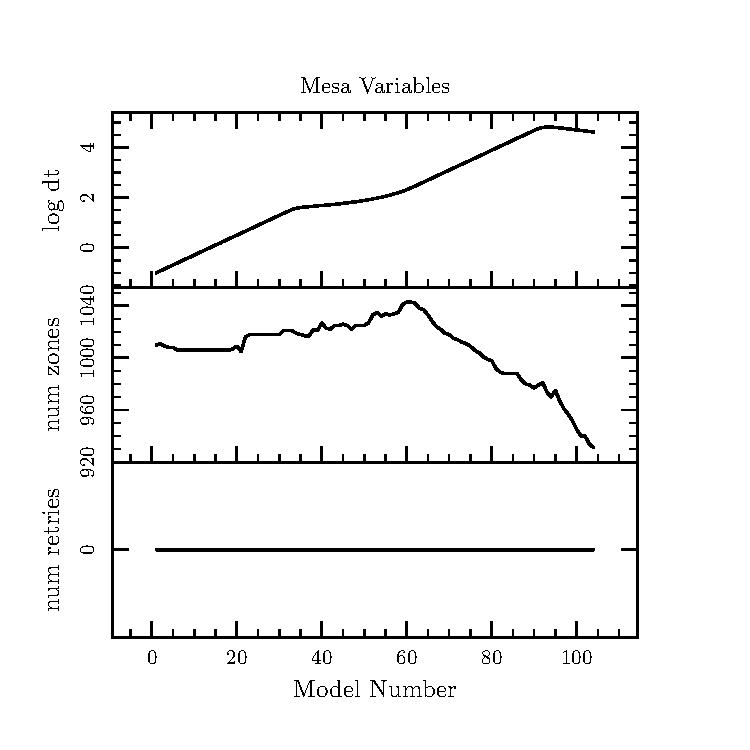
\includegraphics[width = 5in]{/Users/jaredbrooks/high_mass/plots_out/Mesa_Variables.pdf}
          \caption{\texttt{MESA} variables plotted against model number show how hard \texttt{MESA} is working}
          \label{fig:5}
        \end{figure}


\end{document}
